\documentclass[12pt,letterpaper]{article}

% ===== Encoding and fonts =====
\usepackage[utf8]{inputenc}
\usepackage[T1]{fontenc}
\usepackage{mathptmx}
\usepackage{helvet}
\usepackage{courier}

% ===== Page geometry (zero margins) =====
\usepackage[top=0bp,bottom=0bp,left=0bp,right=0bp,headheight=0bp,headsep=0bp,footskip=0bp,paperwidth=612.00bp,paperheight=792.00bp]{geometry}

% ===== Packages =====
\usepackage[dvipsnames,svgnames,x11names]{xcolor}
\usepackage{graphicx}
\usepackage{tikz}
\usepackage{float}
\usepackage{amsmath}
\usepackage{amssymb}
\usepackage[normalem]{ulem}  % for \uline (underline)

% ===== No default spacing =====
\setlength{\parindent}{0pt}
\setlength{\parskip}{0pt}
\pagestyle{empty}

% ===== Currency symbols =====
\usepackage{textcomp}
\newcommand{\rupee}{\textrm{Rs.}}

% ===== Custom colours =====
\definecolor{pdfcolor1}{RGB}{0,116,185}
\definecolor{pdfcolor2}{RGB}{175,175,175}
\definecolor{pdfcolor3}{RGB}{232,232,232}

\begin{document}

\noindent
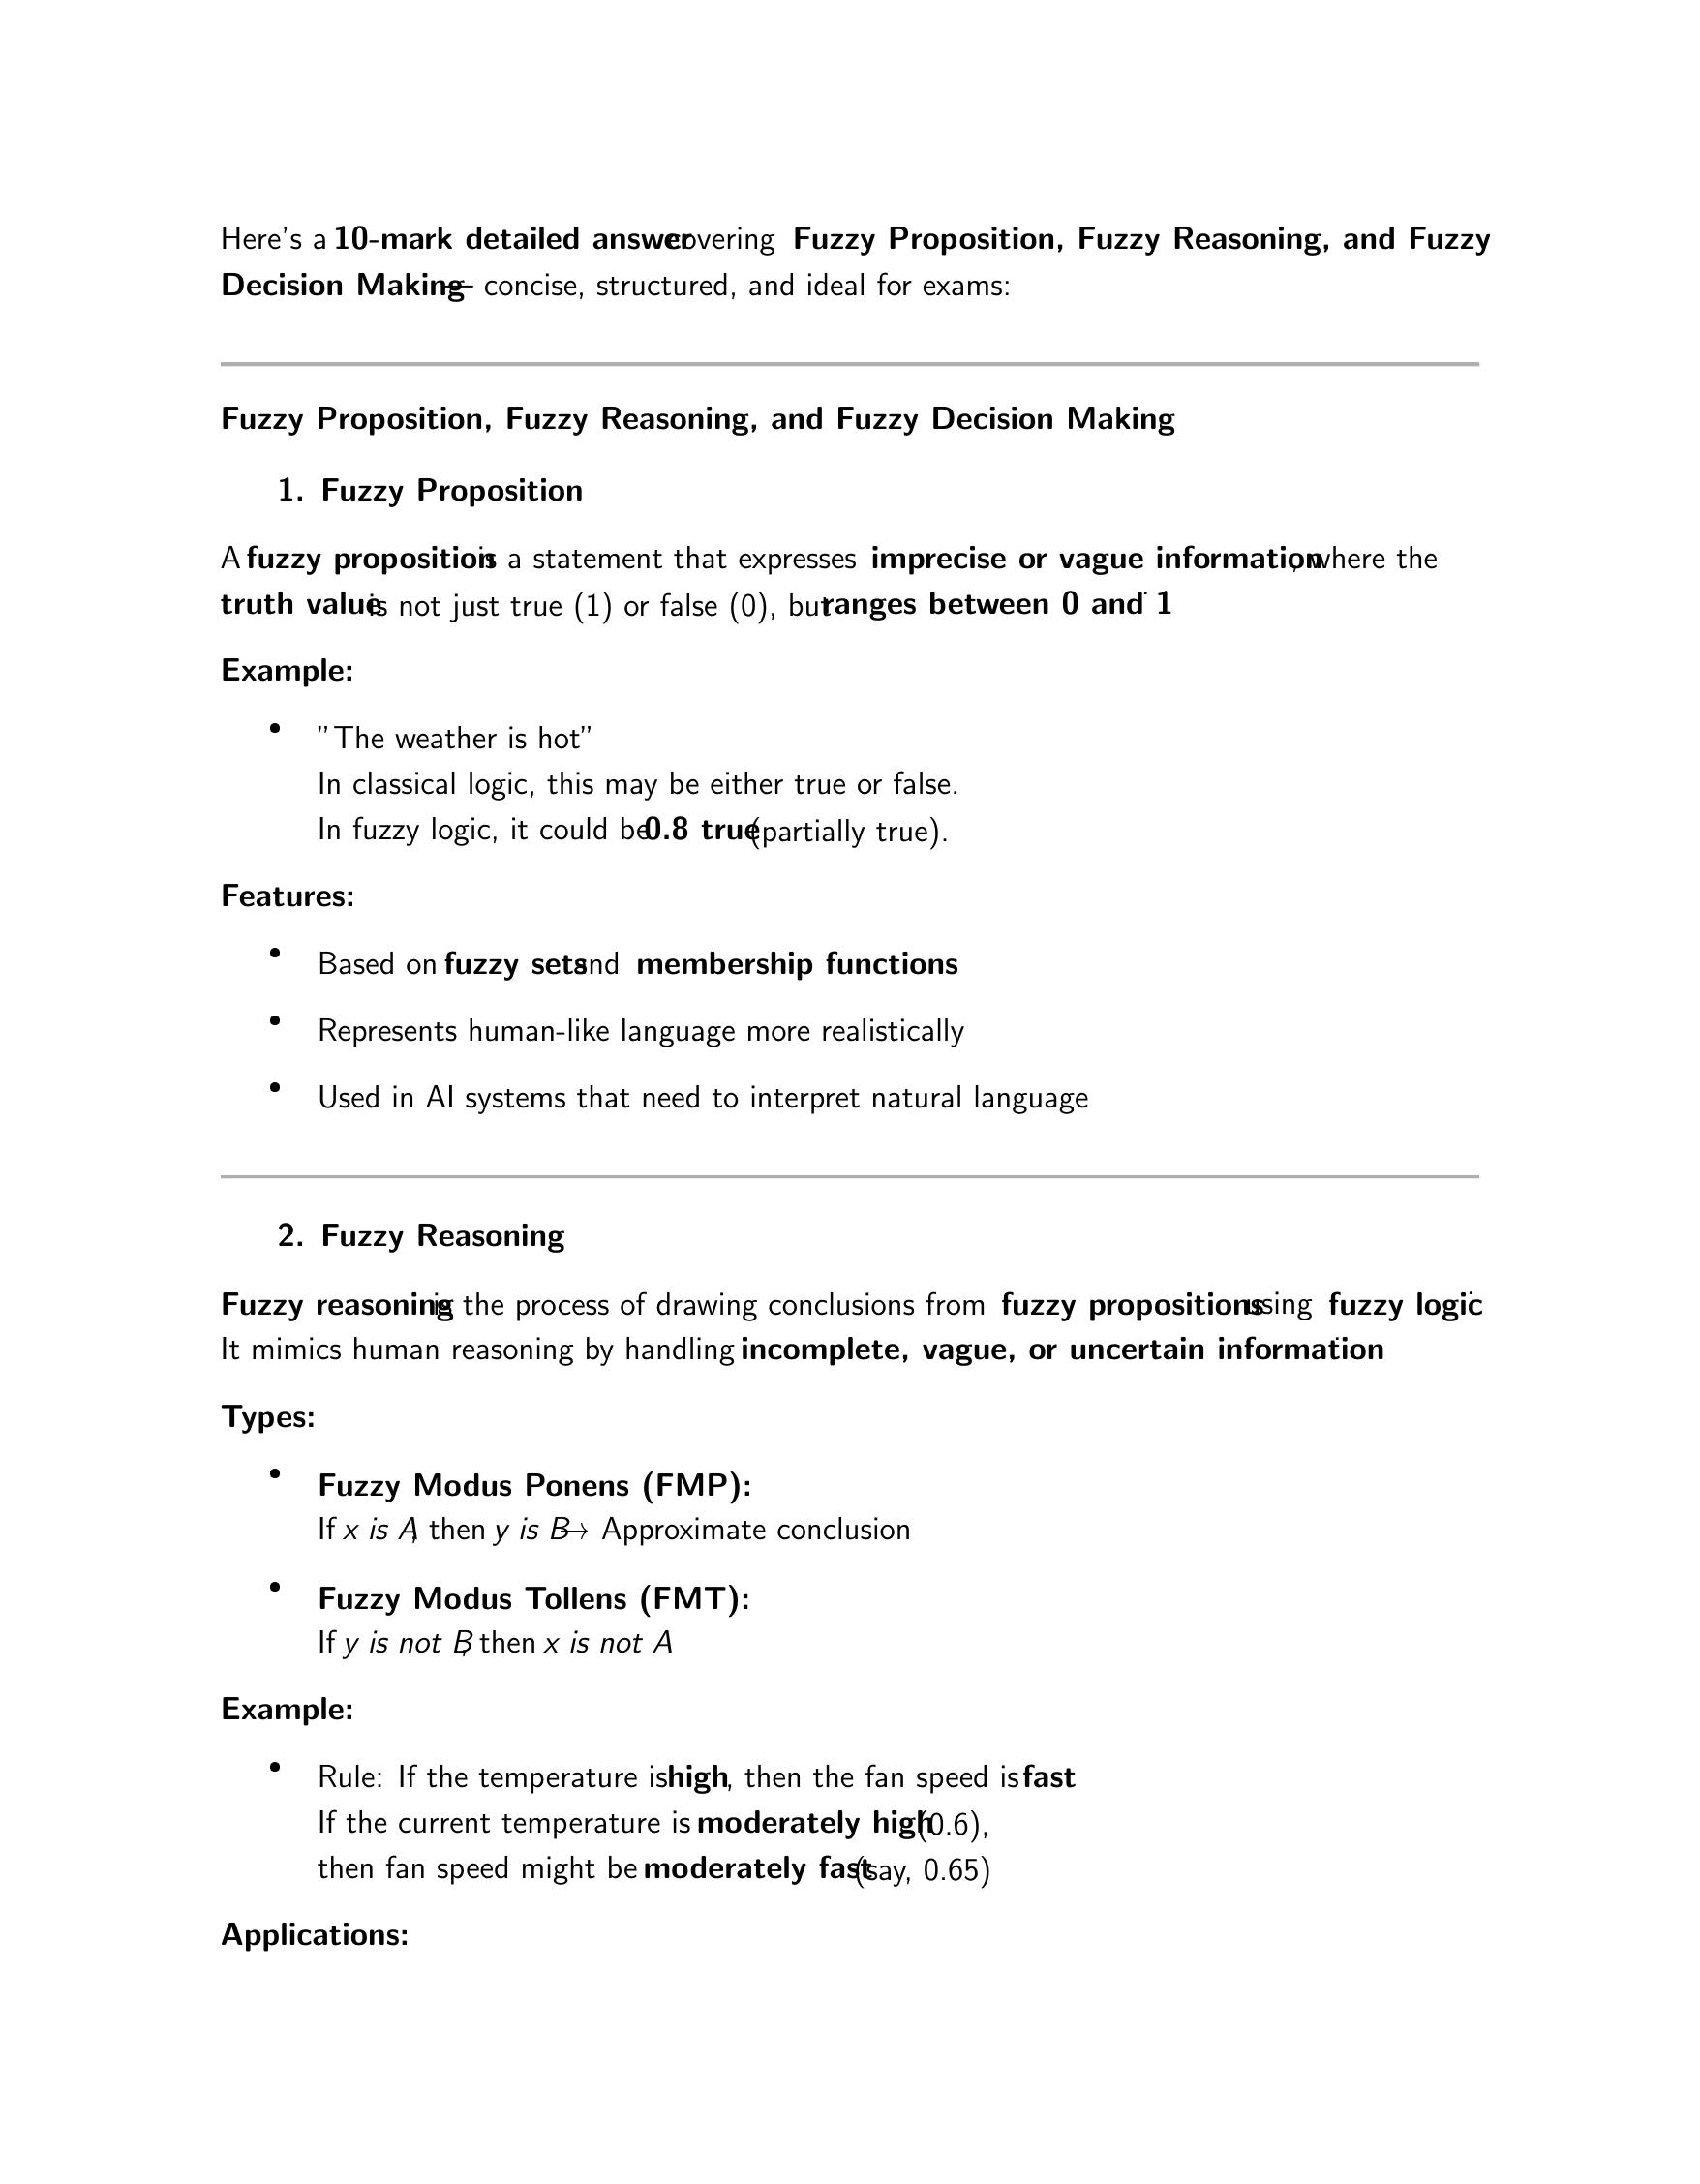
\begin{tikzpicture}[x=1bp,y=-1bp,inner sep=0pt,outer sep=0pt]
  \useasboundingbox (0,0) rectangle (612.00,792.00);
  \fill[fill=pdfcolor2] (72.00,124.80) rectangle (540.00,126.25);
  \fill[fill=pdfcolor2] (72.26,124.85) rectangle (539.97,125.09);
  \fill[fill=pdfcolor2] (72.02,125.09) rectangle (72.26,126.05);
  \fill[fill=pdfcolor3] (539.98,125.09) rectangle (540.22,126.05);
  \fill[fill=pdfcolor3] (72.26,126.05) rectangle (539.97,126.29);
  \fill[fill=pdfcolor2] (72.00,426.95) rectangle (540.00,428.40);
  \fill[fill=pdfcolor2] (72.26,427.08) rectangle (539.97,427.32);
  \fill[fill=pdfcolor2] (72.02,427.32) rectangle (72.26,428.28);
  \fill[fill=pdfcolor3] (539.98,427.32) rectangle (540.22,428.28);
  \fill[fill=pdfcolor3] (72.26,428.28) rectangle (539.97,428.52);
  \node[anchor=north west,inner sep=0pt,outer sep=0pt] at (72.02,74.54) {\textsf{{\fontsize{12.0bp}{14.4bp}\selectfont Here's a }}};
  \node[anchor=north west,inner sep=0pt,outer sep=0pt] at (114.05,74.54) {\textsf{{\fontsize{12.0bp}{14.4bp}\selectfont \textbf{10-mark detailed answer}}}};
  \node[anchor=north west,inner sep=0pt,outer sep=0pt] at (238.18,74.54) {\textsf{{\fontsize{12.0bp}{14.4bp}\selectfont  covering }}};
  \node[anchor=north west,inner sep=0pt,outer sep=0pt] at (284.76,74.54) {\textsf{{\fontsize{12.0bp}{14.4bp}\selectfont \textbf{Fuzzy Proposition, Fuzzy Reasoning, and Fuzzy }}}};
  \node[anchor=north west,inner sep=0pt,outer sep=0pt] at (72.02,91.58) {\textsf{{\fontsize{12.0bp}{14.4bp}\selectfont \textbf{Decision Making}}}};
  \node[anchor=north west,inner sep=0pt,outer sep=0pt] at (154.37,91.58) {\textsf{{\fontsize{12.0bp}{14.4bp}\selectfont  --- concise, structured, and ideal for exams: }}};
  \node[anchor=north west,inner sep=0pt,outer sep=0pt] at (72.02,141.53) {\textsf{{\fontsize{12.0bp}{14.4bp}\selectfont \textbf{Fuzzy Proposition, Fuzzy Reasoning, and Fuzzy Decision Making }}}};
  \node[anchor=north west,inner sep=0pt,outer sep=0pt] at (72.02,167.62) {\textsf{{\fontsize{12.0bp}{14.4bp}\selectfont \textcolor{pdfcolor1}{ }}}};
  \node[anchor=north west,inner sep=0pt,outer sep=0pt] at (88.82,167.93) {\textsf{{\fontsize{12.0bp}{14.4bp}\selectfont \textbf{ 1. Fuzzy Proposition }}}};
  \node[anchor=north west,inner sep=0pt,outer sep=0pt] at (72.02,193.13) {\textsf{{\fontsize{12.0bp}{14.4bp}\selectfont A }}};
  \node[anchor=north west,inner sep=0pt,outer sep=0pt] at (81.62,193.13) {\textsf{{\fontsize{12.0bp}{14.4bp}\selectfont \textbf{fuzzy proposition}}}};
  \node[anchor=north west,inner sep=0pt,outer sep=0pt] at (167.59,193.13) {\textsf{{\fontsize{12.0bp}{14.4bp}\selectfont  is a statement that expresses }}};
  \node[anchor=north west,inner sep=0pt,outer sep=0pt] at (314.04,193.13) {\textsf{{\fontsize{12.0bp}{14.4bp}\selectfont \textbf{imprecise or vague information}}}};
  \node[anchor=north west,inner sep=0pt,outer sep=0pt] at (469.87,193.13) {\textsf{{\fontsize{12.0bp}{14.4bp}\selectfont , where the }}};
  \node[anchor=north west,inner sep=0pt,outer sep=0pt] at (72.02,210.19) {\textsf{{\fontsize{12.0bp}{14.4bp}\selectfont \textbf{truth value}}}};
  \node[anchor=north west,inner sep=0pt,outer sep=0pt] at (127.01,210.19) {\textsf{{\fontsize{12.0bp}{14.4bp}\selectfont  is not just true (1) or false (0), but }}};
  \node[anchor=north west,inner sep=0pt,outer sep=0pt] at (295.80,210.19) {\textsf{{\fontsize{12.0bp}{14.4bp}\selectfont \textbf{ranges between 0 and 1}}}};
  \node[anchor=north west,inner sep=0pt,outer sep=0pt] at (414.41,210.19) {\textsf{{\fontsize{12.0bp}{14.4bp}\selectfont . }}};
  \node[anchor=north west,inner sep=0pt,outer sep=0pt] at (72.02,235.15) {\textsf{{\fontsize{12.0bp}{14.4bp}\selectfont \textbf{Example: }}}};
  \node[anchor=north west,inner sep=0pt,outer sep=0pt] at (90.02,258.98) {{\fontsize{10.1bp}{12.1bp}\selectfont •}};
  \node[anchor=north west,inner sep=0pt,outer sep=0pt] at (94.61,258.27) {\textsf{{\fontsize{10.1bp}{12.1bp}\selectfont  }}};
  \node[anchor=north west,inner sep=0pt,outer sep=0pt] at (108.05,260.11) {\textsf{{\fontsize{12.0bp}{14.4bp}\selectfont ''The weather is hot'' }}};
  \node[anchor=north west,inner sep=0pt,outer sep=0pt] at (108.05,277.15) {\textsf{{\fontsize{12.0bp}{14.4bp}\selectfont In classical logic, this may be either true or false. }}};
  \node[anchor=north west,inner sep=0pt,outer sep=0pt] at (108.05,293.98) {\textsf{{\fontsize{12.0bp}{14.4bp}\selectfont In fuzzy logic, it could be }}};
  \node[anchor=north west,inner sep=0pt,outer sep=0pt] at (229.54,293.98) {\textsf{{\fontsize{12.0bp}{14.4bp}\selectfont \textbf{0.8 true}}}};
  \node[anchor=north west,inner sep=0pt,outer sep=0pt] at (268.66,293.98) {\textsf{{\fontsize{12.0bp}{14.4bp}\selectfont  (partially true). }}};
  \node[anchor=north west,inner sep=0pt,outer sep=0pt] at (72.02,318.94) {\textsf{{\fontsize{12.0bp}{14.4bp}\selectfont \textbf{Features: }}}};
  \node[anchor=north west,inner sep=0pt,outer sep=0pt] at (90.02,342.77) {{\fontsize{10.1bp}{12.1bp}\selectfont •}};
  \node[anchor=north west,inner sep=0pt,outer sep=0pt] at (94.61,342.06) {\textsf{{\fontsize{10.1bp}{12.1bp}\selectfont  }}};
  \node[anchor=north west,inner sep=0pt,outer sep=0pt] at (108.05,343.90) {\textsf{{\fontsize{12.0bp}{14.4bp}\selectfont Based on }}};
  \node[anchor=north west,inner sep=0pt,outer sep=0pt] at (155.11,343.90) {\textsf{{\fontsize{12.0bp}{14.4bp}\selectfont \textbf{fuzzy sets}}}};
  \node[anchor=north west,inner sep=0pt,outer sep=0pt] at (203.11,343.90) {\textsf{{\fontsize{12.0bp}{14.4bp}\selectfont  and }}};
  \node[anchor=north west,inner sep=0pt,outer sep=0pt] at (226.66,343.90) {\textsf{{\fontsize{12.0bp}{14.4bp}\selectfont \textbf{membership functions}}}};
  \node[anchor=north west,inner sep=0pt,outer sep=0pt] at (338.76,343.90) {\textsf{{\fontsize{12.0bp}{14.4bp}\selectfont  }}};
  \node[anchor=north west,inner sep=0pt,outer sep=0pt] at (90.02,367.75) {{\fontsize{10.1bp}{12.1bp}\selectfont •}};
  \node[anchor=north west,inner sep=0pt,outer sep=0pt] at (94.61,367.04) {\textsf{{\fontsize{10.1bp}{12.1bp}\selectfont  }}};
  \node[anchor=north west,inner sep=0pt,outer sep=0pt] at (108.05,368.88) {\textsf{{\fontsize{12.0bp}{14.4bp}\selectfont Represents human-like language more realistically }}};
  \node[anchor=north west,inner sep=0pt,outer sep=0pt] at (90.02,392.71) {{\fontsize{10.1bp}{12.1bp}\selectfont •}};
  \node[anchor=north west,inner sep=0pt,outer sep=0pt] at (94.61,392.00) {\textsf{{\fontsize{10.1bp}{12.1bp}\selectfont  }}};
  \node[anchor=north west,inner sep=0pt,outer sep=0pt] at (108.05,393.84) {\textsf{{\fontsize{12.0bp}{14.4bp}\selectfont Used in AI systems that need to interpret natural language }}};
  \node[anchor=north west,inner sep=0pt,outer sep=0pt] at (72.02,444.91) {\textsf{{\fontsize{12.0bp}{14.4bp}\selectfont \textcolor{pdfcolor1}{ }}}};
  \node[anchor=north west,inner sep=0pt,outer sep=0pt] at (88.82,445.22) {\textsf{{\fontsize{12.0bp}{14.4bp}\selectfont \textbf{ 2. Fuzzy Reasoning }}}};
  \node[anchor=north west,inner sep=0pt,outer sep=0pt] at (72.02,470.66) {\textsf{{\fontsize{12.0bp}{14.4bp}\selectfont \textbf{Fuzzy reasoning}}}};
  \node[anchor=north west,inner sep=0pt,outer sep=0pt] at (151.01,470.66) {\textsf{{\fontsize{12.0bp}{14.4bp}\selectfont  is the process of drawing conclusions from }}};
  \node[anchor=north west,inner sep=0pt,outer sep=0pt] at (362.30,470.66) {\textsf{{\fontsize{12.0bp}{14.4bp}\selectfont \textbf{fuzzy propositions}}}};
  \node[anchor=north west,inner sep=0pt,outer sep=0pt] at (453.05,470.66) {\textsf{{\fontsize{12.0bp}{14.4bp}\selectfont  using }}};
  \node[anchor=north west,inner sep=0pt,outer sep=0pt] at (484.03,470.66) {\textsf{{\fontsize{12.0bp}{14.4bp}\selectfont \textbf{fuzzy logic}}}};
  \node[anchor=north west,inner sep=0pt,outer sep=0pt] at (535.42,470.66) {\textsf{{\fontsize{12.0bp}{14.4bp}\selectfont . }}};
  \node[anchor=north west,inner sep=0pt,outer sep=0pt] at (72.02,487.46) {\textsf{{\fontsize{12.0bp}{14.4bp}\selectfont It mimics human reasoning by handling }}};
  \node[anchor=north west,inner sep=0pt,outer sep=0pt] at (265.54,487.46) {\textsf{{\fontsize{12.0bp}{14.4bp}\selectfont \textbf{incomplete, vague, or uncertain information}}}};
  \node[anchor=north west,inner sep=0pt,outer sep=0pt] at (485.71,487.46) {\textsf{{\fontsize{12.0bp}{14.4bp}\selectfont . }}};
  \node[anchor=north west,inner sep=0pt,outer sep=0pt] at (72.02,512.42) {\textsf{{\fontsize{12.0bp}{14.4bp}\selectfont \textbf{Types: }}}};
  \node[anchor=north west,inner sep=0pt,outer sep=0pt] at (90.02,536.28) {{\fontsize{10.1bp}{12.1bp}\selectfont •}};
  \node[anchor=north west,inner sep=0pt,outer sep=0pt] at (94.61,535.57) {\textsf{{\fontsize{10.1bp}{12.1bp}\selectfont  }}};
  \node[anchor=north west,inner sep=0pt,outer sep=0pt] at (108.05,537.41) {\textsf{{\fontsize{12.0bp}{14.4bp}\selectfont \textbf{Fuzzy Modus Ponens (FMP):}}}};
  \node[anchor=north west,inner sep=0pt,outer sep=0pt] at (247.54,537.41) {\textsf{{\fontsize{12.0bp}{14.4bp}\selectfont  }}};
  \node[anchor=north west,inner sep=0pt,outer sep=0pt] at (108.05,554.45) {\textsf{{\fontsize{12.0bp}{14.4bp}\selectfont If }}};
  \node[anchor=north west,inner sep=0pt,outer sep=0pt] at (117.41,554.45) {\textsf{{\fontsize{12.0bp}{14.4bp}\selectfont \textit{x is A}}}};
  \node[anchor=north west,inner sep=0pt,outer sep=0pt] at (142.37,554.45) {\textsf{{\fontsize{12.0bp}{14.4bp}\selectfont , then }}};
  \node[anchor=north west,inner sep=0pt,outer sep=0pt] at (173.35,554.45) {\textsf{{\fontsize{12.0bp}{14.4bp}\selectfont \textit{y is B}}}};
  \node[anchor=north west,inner sep=0pt,outer sep=0pt] at (198.07,554.45) {\textsf{{\fontsize{12.0bp}{14.4bp}\selectfont  → Approximate conclusion }}};
  \node[anchor=north west,inner sep=0pt,outer sep=0pt] at (90.02,578.28) {{\fontsize{10.1bp}{12.1bp}\selectfont •}};
  \node[anchor=north west,inner sep=0pt,outer sep=0pt] at (94.61,577.57) {\textsf{{\fontsize{10.1bp}{12.1bp}\selectfont  }}};
  \node[anchor=north west,inner sep=0pt,outer sep=0pt] at (108.05,579.41) {\textsf{{\fontsize{12.0bp}{14.4bp}\selectfont \textbf{Fuzzy Modus Tollens (FMT):}}}};
  \node[anchor=north west,inner sep=0pt,outer sep=0pt] at (245.14,579.41) {\textsf{{\fontsize{12.0bp}{14.4bp}\selectfont  }}};
  \node[anchor=north west,inner sep=0pt,outer sep=0pt] at (108.05,596.45) {\textsf{{\fontsize{12.0bp}{14.4bp}\selectfont If }}};
  \node[anchor=north west,inner sep=0pt,outer sep=0pt] at (117.41,596.45) {\textsf{{\fontsize{12.0bp}{14.4bp}\selectfont \textit{y is not B}}}};
  \node[anchor=north west,inner sep=0pt,outer sep=0pt] at (161.11,596.45) {\textsf{{\fontsize{12.0bp}{14.4bp}\selectfont , then }}};
  \node[anchor=north west,inner sep=0pt,outer sep=0pt] at (192.07,596.45) {\textsf{{\fontsize{12.0bp}{14.4bp}\selectfont \textit{x is not A}}}};
  \node[anchor=north west,inner sep=0pt,outer sep=0pt] at (236.26,596.45) {\textsf{{\fontsize{12.0bp}{14.4bp}\selectfont  }}};
  \node[anchor=north west,inner sep=0pt,outer sep=0pt] at (72.02,621.43) {\textsf{{\fontsize{12.0bp}{14.4bp}\selectfont \textbf{Example: }}}};
  \node[anchor=north west,inner sep=0pt,outer sep=0pt] at (90.02,645.26) {{\fontsize{10.1bp}{12.1bp}\selectfont •}};
  \node[anchor=north west,inner sep=0pt,outer sep=0pt] at (94.61,644.55) {\textsf{{\fontsize{10.1bp}{12.1bp}\selectfont  }}};
  \node[anchor=north west,inner sep=0pt,outer sep=0pt] at (108.05,646.39) {\textsf{{\fontsize{12.0bp}{14.4bp}\selectfont Rule: If the temperature is }}};
  \node[anchor=north west,inner sep=0pt,outer sep=0pt] at (238.18,646.39) {\textsf{{\fontsize{12.0bp}{14.4bp}\selectfont \textbf{high}}}};
  \node[anchor=north west,inner sep=0pt,outer sep=0pt] at (259.78,646.39) {\textsf{{\fontsize{12.0bp}{14.4bp}\selectfont , then the fan speed is }}};
  \node[anchor=north west,inner sep=0pt,outer sep=0pt] at (370.22,646.39) {\textsf{{\fontsize{12.0bp}{14.4bp}\selectfont \textbf{fast}}}};
  \node[anchor=north west,inner sep=0pt,outer sep=0pt] at (388.70,646.39) {\textsf{{\fontsize{12.0bp}{14.4bp}\selectfont  }}};
  \node[anchor=north west,inner sep=0pt,outer sep=0pt] at (108.05,663.43) {\textsf{{\fontsize{12.0bp}{14.4bp}\selectfont If the current temperature is }}};
  \node[anchor=north west,inner sep=0pt,outer sep=0pt] at (249.22,663.43) {\textsf{{\fontsize{12.0bp}{14.4bp}\selectfont \textbf{moderately high}}}};
  \node[anchor=north west,inner sep=0pt,outer sep=0pt] at (330.84,663.43) {\textsf{{\fontsize{12.0bp}{14.4bp}\selectfont  (0.6), }}};
  \node[anchor=north west,inner sep=0pt,outer sep=0pt] at (108.05,680.23) {\textsf{{\fontsize{12.0bp}{14.4bp}\selectfont then fan speed might be }}};
  \node[anchor=north west,inner sep=0pt,outer sep=0pt] at (229.30,680.23) {\textsf{{\fontsize{12.0bp}{14.4bp}\selectfont \textbf{moderately fast}}}};
  \node[anchor=north west,inner sep=0pt,outer sep=0pt] at (307.56,680.23) {\textsf{{\fontsize{12.0bp}{14.4bp}\selectfont  (say, 0.65) }}};
  \node[anchor=north west,inner sep=0pt,outer sep=0pt] at (72.02,705.22) {\textsf{{\fontsize{12.0bp}{14.4bp}\selectfont \textbf{Applications: }}}};
\end{tikzpicture}
\newpage
\noindent
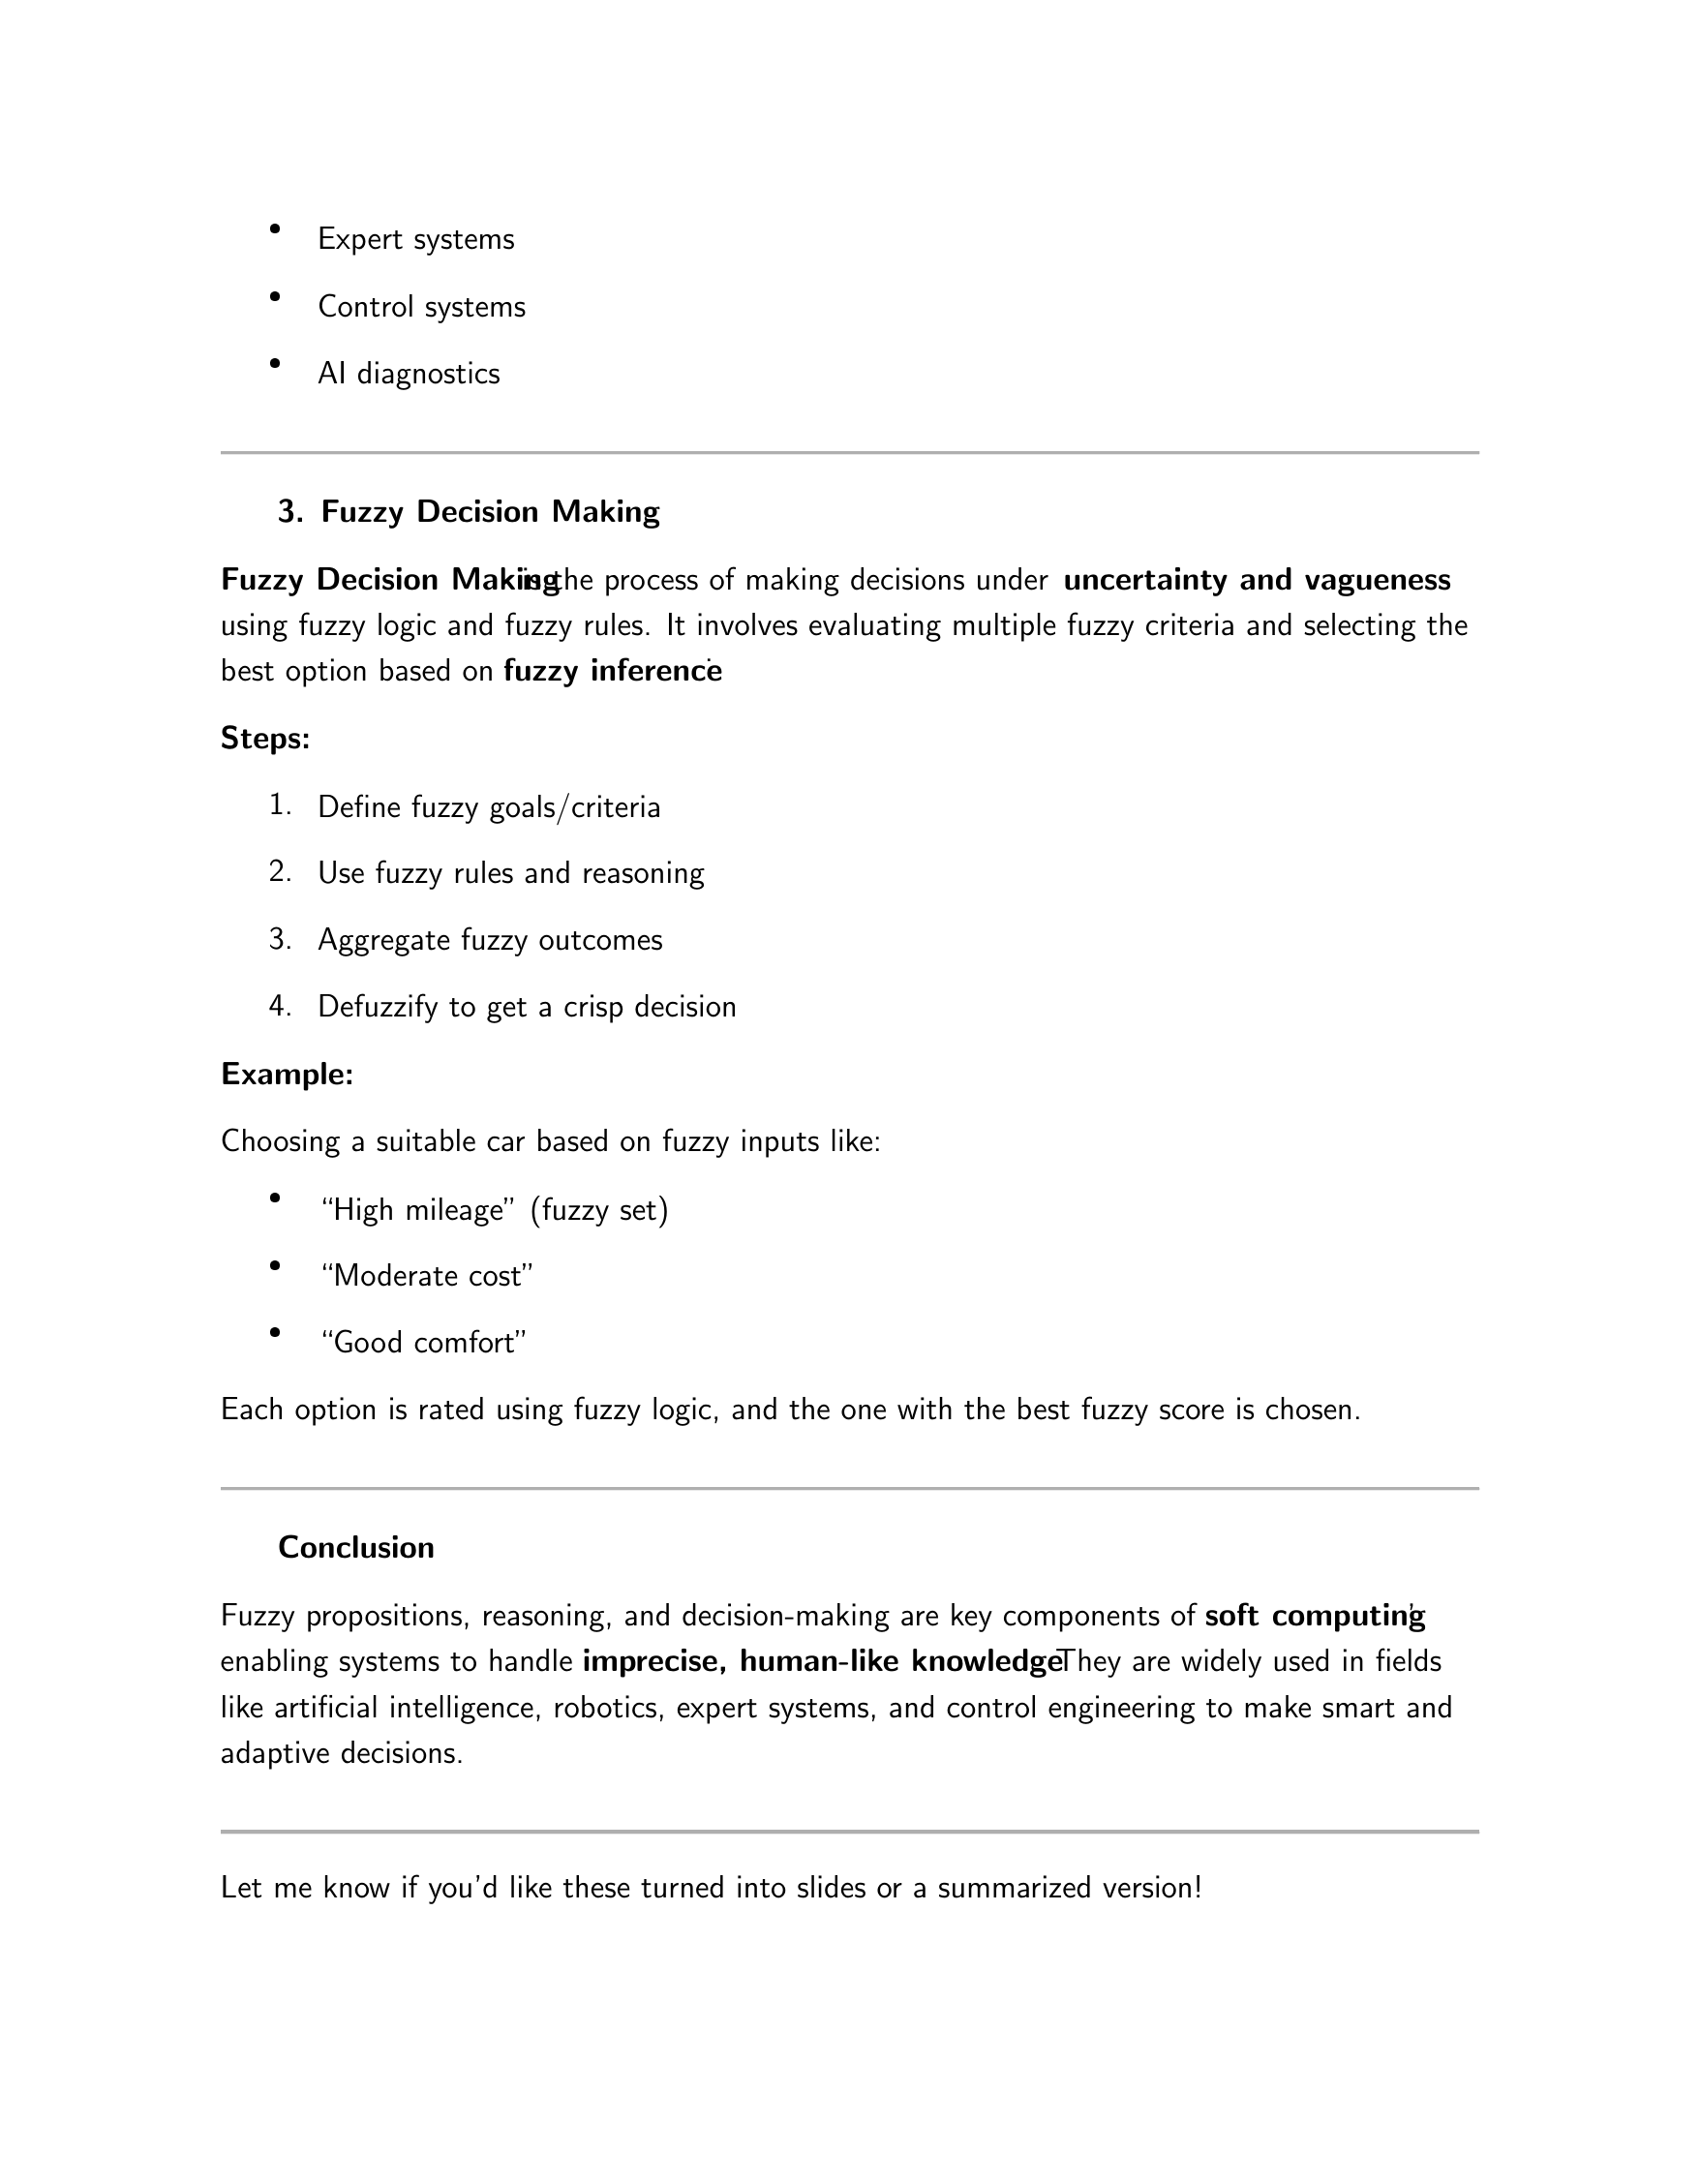
\begin{tikzpicture}[x=1bp,y=-1bp,inner sep=0pt,outer sep=0pt]
  \useasboundingbox (0,0) rectangle (612.00,792.00);
  \fill[fill=pdfcolor2] (72.00,157.70) rectangle (540.00,159.10);
  \fill[fill=pdfcolor2] (72.26,157.73) rectangle (539.97,157.97);
  \fill[fill=pdfcolor2] (72.02,157.97) rectangle (72.26,158.93);
  \fill[fill=pdfcolor3] (539.98,157.97) rectangle (540.22,158.93);
  \fill[fill=pdfcolor3] (72.26,158.93) rectangle (539.97,159.17);
  \fill[fill=pdfcolor2] (72.00,542.90) rectangle (540.00,544.30);
  \fill[fill=pdfcolor2] (72.26,543.05) rectangle (539.97,543.29);
  \fill[fill=pdfcolor2] (72.02,543.29) rectangle (72.26,544.25);
  \fill[fill=pdfcolor3] (539.98,543.29) rectangle (540.22,544.25);
  \fill[fill=pdfcolor3] (72.26,544.25) rectangle (539.97,544.49);
  \fill[fill=pdfcolor2] (72.00,670.55) rectangle (540.00,672.00);
  \fill[fill=pdfcolor2] (72.26,670.75) rectangle (539.97,670.99);
  \fill[fill=pdfcolor2] (72.02,670.99) rectangle (72.26,671.95);
  \fill[fill=pdfcolor3] (539.98,670.99) rectangle (540.22,671.95);
  \fill[fill=pdfcolor3] (72.26,671.95) rectangle (539.97,672.19);
  \node[anchor=north west,inner sep=0pt,outer sep=0pt] at (90.02,73.41) {{\fontsize{10.1bp}{12.1bp}\selectfont •}};
  \node[anchor=north west,inner sep=0pt,outer sep=0pt] at (94.61,72.70) {\textsf{{\fontsize{10.1bp}{12.1bp}\selectfont  }}};
  \node[anchor=north west,inner sep=0pt,outer sep=0pt] at (108.05,74.54) {\textsf{{\fontsize{12.0bp}{14.4bp}\selectfont Expert systems }}};
  \node[anchor=north west,inner sep=0pt,outer sep=0pt] at (90.02,98.37) {{\fontsize{10.1bp}{12.1bp}\selectfont •}};
  \node[anchor=north west,inner sep=0pt,outer sep=0pt] at (94.61,97.66) {\textsf{{\fontsize{10.1bp}{12.1bp}\selectfont  }}};
  \node[anchor=north west,inner sep=0pt,outer sep=0pt] at (108.05,99.50) {\textsf{{\fontsize{12.0bp}{14.4bp}\selectfont Control systems }}};
  \node[anchor=north west,inner sep=0pt,outer sep=0pt] at (90.02,123.36) {{\fontsize{10.1bp}{12.1bp}\selectfont •}};
  \node[anchor=north west,inner sep=0pt,outer sep=0pt] at (94.61,122.65) {\textsf{{\fontsize{10.1bp}{12.1bp}\selectfont  }}};
  \node[anchor=north west,inner sep=0pt,outer sep=0pt] at (108.05,124.49) {\textsf{{\fontsize{12.0bp}{14.4bp}\selectfont AI diagnostics }}};
  \node[anchor=north west,inner sep=0pt,outer sep=0pt] at (72.02,175.54) {\textsf{{\fontsize{12.0bp}{14.4bp}\selectfont \textcolor{pdfcolor1}{ }}}};
  \node[anchor=north west,inner sep=0pt,outer sep=0pt] at (88.82,175.85) {\textsf{{\fontsize{12.0bp}{14.4bp}\selectfont \textbf{ 3. Fuzzy Decision Making }}}};
  \node[anchor=north west,inner sep=0pt,outer sep=0pt] at (72.02,201.07) {\textsf{{\fontsize{12.0bp}{14.4bp}\selectfont \textbf{Fuzzy Decision Making}}}};
  \node[anchor=north west,inner sep=0pt,outer sep=0pt] at (184.15,201.07) {\textsf{{\fontsize{12.0bp}{14.4bp}\selectfont  is the process of making decisions under }}};
  \node[anchor=north west,inner sep=0pt,outer sep=0pt] at (385.58,201.07) {\textsf{{\fontsize{12.0bp}{14.4bp}\selectfont \textbf{uncertainty and vagueness}}}};
  \node[anchor=north west,inner sep=0pt,outer sep=0pt] at (519.07,201.07) {\textsf{{\fontsize{12.0bp}{14.4bp}\selectfont  }}};
  \node[anchor=north west,inner sep=0pt,outer sep=0pt] at (72.02,218.11) {\textsf{{\fontsize{12.0bp}{14.4bp}\selectfont using fuzzy logic and fuzzy rules. It involves evaluating multiple fuzzy criteria and selecting the }}};
  \node[anchor=north west,inner sep=0pt,outer sep=0pt] at (72.02,235.15) {\textsf{{\fontsize{12.0bp}{14.4bp}\selectfont best option based on }}};
  \node[anchor=north west,inner sep=0pt,outer sep=0pt] at (177.19,235.15) {\textsf{{\fontsize{12.0bp}{14.4bp}\selectfont \textbf{fuzzy inference}}}};
  \node[anchor=north west,inner sep=0pt,outer sep=0pt] at (252.10,235.15) {\textsf{{\fontsize{12.0bp}{14.4bp}\selectfont . }}};
  \node[anchor=north west,inner sep=0pt,outer sep=0pt] at (72.02,260.11) {\textsf{{\fontsize{12.0bp}{14.4bp}\selectfont \textbf{Steps: }}}};
  \node[anchor=north west,inner sep=0pt,outer sep=0pt] at (90.02,285.10) {\textsf{{\fontsize{12.0bp}{14.4bp}\selectfont 1.}}};
  \node[anchor=north west,inner sep=0pt,outer sep=0pt] at (99.17,281.20) {\textsf{{\fontsize{12.0bp}{14.4bp}\selectfont  }}};
  \node[anchor=north west,inner sep=0pt,outer sep=0pt] at (108.05,285.10) {\textsf{{\fontsize{12.0bp}{14.4bp}\selectfont Define fuzzy goals/criteria }}};
  \node[anchor=north west,inner sep=0pt,outer sep=0pt] at (90.02,310.06) {\textsf{{\fontsize{12.0bp}{14.4bp}\selectfont 2.}}};
  \node[anchor=north west,inner sep=0pt,outer sep=0pt] at (99.17,306.16) {\textsf{{\fontsize{12.0bp}{14.4bp}\selectfont  }}};
  \node[anchor=north west,inner sep=0pt,outer sep=0pt] at (108.05,310.06) {\textsf{{\fontsize{12.0bp}{14.4bp}\selectfont Use fuzzy rules and reasoning }}};
  \node[anchor=north west,inner sep=0pt,outer sep=0pt] at (90.02,335.02) {\textsf{{\fontsize{12.0bp}{14.4bp}\selectfont 3.}}};
  \node[anchor=north west,inner sep=0pt,outer sep=0pt] at (99.17,331.12) {\textsf{{\fontsize{12.0bp}{14.4bp}\selectfont  }}};
  \node[anchor=north west,inner sep=0pt,outer sep=0pt] at (108.05,335.02) {\textsf{{\fontsize{12.0bp}{14.4bp}\selectfont Aggregate fuzzy outcomes }}};
  \node[anchor=north west,inner sep=0pt,outer sep=0pt] at (90.02,359.98) {\textsf{{\fontsize{12.0bp}{14.4bp}\selectfont 4.}}};
  \node[anchor=north west,inner sep=0pt,outer sep=0pt] at (99.17,356.08) {\textsf{{\fontsize{12.0bp}{14.4bp}\selectfont  }}};
  \node[anchor=north west,inner sep=0pt,outer sep=0pt] at (108.05,359.98) {\textsf{{\fontsize{12.0bp}{14.4bp}\selectfont Defuzzify to get a crisp decision }}};
  \node[anchor=north west,inner sep=0pt,outer sep=0pt] at (72.02,384.96) {\textsf{{\fontsize{12.0bp}{14.4bp}\selectfont \textbf{Example: }}}};
  \node[anchor=north west,inner sep=0pt,outer sep=0pt] at (72.02,409.92) {\textsf{{\fontsize{12.0bp}{14.4bp}\selectfont Choosing a suitable car based on fuzzy inputs like: }}};
  \node[anchor=north west,inner sep=0pt,outer sep=0pt] at (90.02,433.75) {{\fontsize{10.1bp}{12.1bp}\selectfont •}};
  \node[anchor=north west,inner sep=0pt,outer sep=0pt] at (94.61,433.04) {\textsf{{\fontsize{10.1bp}{12.1bp}\selectfont  }}};
  \node[anchor=north west,inner sep=0pt,outer sep=0pt] at (108.05,434.88) {\textsf{{\fontsize{12.0bp}{14.4bp}\selectfont “High mileage” (fuzzy set) }}};
  \node[anchor=north west,inner sep=0pt,outer sep=0pt] at (90.02,458.73) {{\fontsize{10.1bp}{12.1bp}\selectfont •}};
  \node[anchor=north west,inner sep=0pt,outer sep=0pt] at (94.61,458.02) {\textsf{{\fontsize{10.1bp}{12.1bp}\selectfont  }}};
  \node[anchor=north west,inner sep=0pt,outer sep=0pt] at (108.05,459.86) {\textsf{{\fontsize{12.0bp}{14.4bp}\selectfont “Moderate cost” }}};
  \node[anchor=north west,inner sep=0pt,outer sep=0pt] at (90.02,483.69) {{\fontsize{10.1bp}{12.1bp}\selectfont •}};
  \node[anchor=north west,inner sep=0pt,outer sep=0pt] at (94.61,482.98) {\textsf{{\fontsize{10.1bp}{12.1bp}\selectfont  }}};
  \node[anchor=north west,inner sep=0pt,outer sep=0pt] at (108.05,484.82) {\textsf{{\fontsize{12.0bp}{14.4bp}\selectfont “Good comfort” }}};
  \node[anchor=north west,inner sep=0pt,outer sep=0pt] at (72.02,509.78) {\textsf{{\fontsize{12.0bp}{14.4bp}\selectfont Each option is rated using fuzzy logic, and the one with the best fuzzy score is chosen. }}};
  \node[anchor=north west,inner sep=0pt,outer sep=0pt] at (72.02,560.86) {\textsf{{\fontsize{12.0bp}{14.4bp}\selectfont \textcolor{pdfcolor1}{ }}}};
  \node[anchor=north west,inner sep=0pt,outer sep=0pt] at (88.82,561.17) {\textsf{{\fontsize{12.0bp}{14.4bp}\selectfont \textbf{ Conclusion }}}};
  \node[anchor=north west,inner sep=0pt,outer sep=0pt] at (72.02,586.37) {\textsf{{\fontsize{12.0bp}{14.4bp}\selectfont Fuzzy propositions, reasoning, and decision-making are key components of }}};
  \node[anchor=north west,inner sep=0pt,outer sep=0pt] at (438.17,586.37) {\textsf{{\fontsize{12.0bp}{14.4bp}\selectfont \textbf{soft computing}}}};
  \node[anchor=north west,inner sep=0pt,outer sep=0pt] at (513.31,586.37) {\textsf{{\fontsize{12.0bp}{14.4bp}\selectfont , }}};
  \node[anchor=north west,inner sep=0pt,outer sep=0pt] at (72.02,603.41) {\textsf{{\fontsize{12.0bp}{14.4bp}\selectfont enabling systems to handle }}};
  \node[anchor=north west,inner sep=0pt,outer sep=0pt] at (206.71,603.41) {\textsf{{\fontsize{12.0bp}{14.4bp}\selectfont \textbf{imprecise, human-like knowledge}}}};
  \node[anchor=north west,inner sep=0pt,outer sep=0pt] at (374.06,603.41) {\textsf{{\fontsize{12.0bp}{14.4bp}\selectfont . They are widely used in fields }}};
  \node[anchor=north west,inner sep=0pt,outer sep=0pt] at (72.02,620.47) {\textsf{{\fontsize{12.0bp}{14.4bp}\selectfont like artificial intelligence, robotics, expert systems, and control engineering to make smart and }}};
  \node[anchor=north west,inner sep=0pt,outer sep=0pt] at (72.02,637.51) {\textsf{{\fontsize{12.0bp}{14.4bp}\selectfont adaptive decisions. }}};
  \node[anchor=north west,inner sep=0pt,outer sep=0pt] at (72.02,687.43) {\textsf{{\fontsize{12.0bp}{14.4bp}\selectfont Let me know if you'd like these turned into slides or a summarized version! }}};
\end{tikzpicture}

\end{document}
